\chapter{Durchführung}

\section{$\alpha_p$-Studie (VR)}
Zur Maximierung der Zugfestigkeit der Legierung Ti-6242 wurde zuerst der Einfluss des $\alpha_p$-Phasenanteils auf die Härte untersucht. Laut \ref{bib:} konnte bei der Legierung IMI834 eine maximale Zugfestigkeit bei einem $\alpha_p$-Anteil von 10--20\% festgestellt werden. \\
Um eine größtmögliche Härtesteigerung gegenüber der as-received-Probe (AR) zu erzielen, wurden vier Proben bei unterschiedlichen Temperaturen $1h$ unterhalb der $\beta$-Transus-Temperatur geglüht und anschließend luftgekühlt (AC: air cooled) (\ref{tab:alphap}). Dabei stellt sich ein bimodales Gefüge ein. Dieser Schritt wurde beim TS-STDA nicht explitit durchgeführt, da der erste Schritt dort gleichzeitig das bimodale Gefüge einstellt und die $\beta$-Phase martensitisch umwandelt. Die vier Proben wurden inklusive einer AR-Probe metallografisch präpariert und ausgewertet.



\begin{table}
		\centering
	\begin{tabular}{|c|c|c|c|}
	\hline 
	Probenbezeichnung & Temperatur [$^\circ C$] & Zeit [$h$] & Abkühlmethode \\ 
	\hline 
	BM990 & 990 & 1 & AC\\ 
	\hline 
	
	BM975 & 975 & 1 & AC\\ 
	\hline 
	BM960 & 960 & 1 & AC\\ 
	\hline 
	\end{tabular} 
	\caption{Wärmebehandlung der $\alpha_p$-Studie}
	\label{tab:alphap}
\end{table}


\section{Martensit-Bildung}

Um Martensit zu bilden wird Ti-64 nach der ersten Wärmebehandlung laut Abbildung \ref{STDA} für $1 min$  bei $930\circ C$ erwärmt und dann  auf Raumtemperatur wassergekühlt. Unter dem Einfluss der Diffusion soll sich die erhaltene und metastabile Beta Phase aus der bimodalen Struktur weiter wachsen. Die kurze Erwärmungszeit soll dafür sorgen, dass die neu gebildeten Beta-Gebiete nicht mit $\beta$-Stabilisatoren, in diesem Fall Vanadium, bereichert  und dadurch stabilisiert werden. Durch das schnelle Abschrecken auf Raumtemperatur wandelt sich das "neue "$\beta$ diffusionslos und lokal in Martensit um.

\begin{figure}[H]
	\centering
	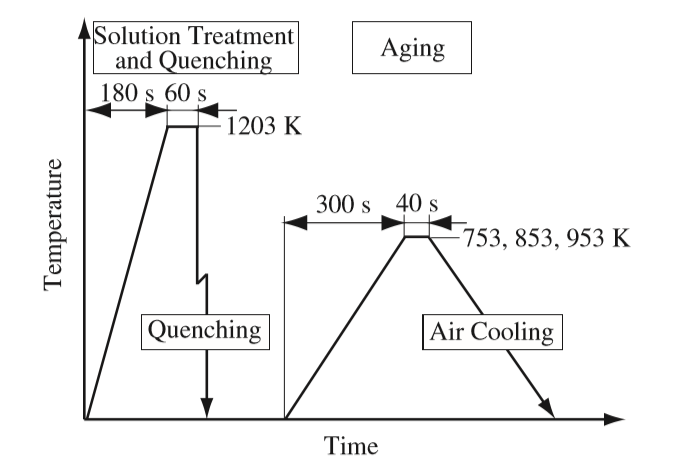
\includegraphics[width=0.9\textwidth]{Bilder/ts-stda}
	\caption{Vorgehensweise nach dem Duplex-Anneal bei STDA für Ti-64 (Strengthening of Ti–6Al–4V Alloy by Short-Time Duplex Heat Treatment)}
	\label{STDA}
\end{figure}

Da die $\beta_{t}$ von Ti-64 niedriger ist als die von Ti-6242, liegt auch ihre Gleichgewichtstemperatur unterhalb der von Ti-6242. Außerdem hat Vanadium im Vergleich zu Molybdän eine größere Diffusionsrate in Titan, was die schnellen Anlasszeiten erklärt[Titan und Titan legierungen, Zwicker]. Deswegen wurden in diesem Schritt die Ti-6242-Proben nach dem Duplex-Glühen für 8 und 16 $min$ jeweils bei $930\circ C$d und $950\circ C$ wärmebehandelt.

Eine bekannte Wärmebehandlung von $\alpha$+$\beta$-Titanlegierungen ist die  \textit{Solution treatment and quenching}, wobei die Titanlegierung direkt von einer Temperatur $T_{1}$ unterhalb  $\beta_{t}$ nach 0,5-1 h abgeschreckt wird. Wie bei der oben beschriebenen Wärmebehandlung stellt sich bei $T_{1}$ ein zweiphasiges Gefüge mit $\alpha_p$ und $\beta$ ein. Die $\beta$-Phase wandelt sich  dann beim Abschrecken martensitisch um und wird $\alpha^\prime$ genannt.(Strengthening of Ti–6Al–4V Alloy by Short-Time Duplex Heat Treatment)
Zum Vergleich zu der studierten Wärmebehandlung werden AR-Proben bei 983°C für 1h erwärmt und wassergekühlt.

\section{Martensit-Zerfall (TJ)}

Weiterhin ist gewünscht die Härte der Legierung zu steigen. Dafür wurde eine Martensit Zerfall erwünscht. Dieses passiert in Transformiertes $\beta$. 

Es kommt zu einer Dekomposition der Martensit, der in $\alpha$ + $\beta$ transformiert. Dadurch, dass Martensit Bildung sich im Nanometer Skala findet, erfolgen mehrere kleine Lamellen. Es herrschen extrem kleine Diffusionsvorgänge. Der Martensit ist also lokal im Gefüge zu finden. Es werden also nicht lange Zeiten gebraucht für die Wärmevorgänge.

Die Probe 983°/1h/AC + 950/16min/WQ ist ausgewählt worden für die nächsten Vorgänge. Dazu wurde eine kleine Studie gemacht. Untersucht wird ob bei zwei verschiedene Temperaturen einen Anstieg an der Härte erbringt. Wir haben uns an das Three Step Short Time Duplex Anneal für Ti-64 Paper von T. Morita, K. Hatsuoka, T. Iizuka und K. Kawasaki orientiert. Die erste Temperatur ist übernommen worden. Für die ersten Proben: 580 C. Und für die zweite Temperatur, sind 30K gestiegen (610C). Untersucht wird, ob ein Unterschied bei einer höheren Temperatur gibt.Für beide Schritte sind kurze Zeiten ausgewählt worden. Für die jeweiligen Temperaturen werden die Proben im Ofen für 8 Minuten bzw. 16 Minuten geglüht. Sie werden danach im Wasser abgekühlt. 

Es ist bekannt, dass bis das innere Teil der Probe die gewünschte Temperatur erreicht, brauch es eine gewisse Zeit. Diese Zeit wird mit 4 Minuten geschätzt. Es besteht die Hoffnung eine Härtesteigerung zu erreichen.



\subsection{Parallelversuch}

Für das $\alpha$´ + Primär-$\alpha$ wird auch ein Martensit Zerfall durchgeführt. Bei diesem Gefüge sieht das Vorgehen ein wenig anders aus. Dadurch das es sich global Martensit gebildet hat, werden hier höhere Zeiten ausgewählt. Für eine Temperatur von 610° werden 16 Minuten und 30 Minuten geschätzt. Es ist erwartet, dass die Proben mehr Zeit für den Zerfall brauchen, da es mehr Martensit gibt. 


\section{Martensit-Zerfall (TJ)}
Weiterhin ist gewünscht die Härte der Legierung zu steigern. Ein Martensit Zerfall wurde den erwünschten Effekt noch steigern. Dieses passiert in der transformierten $\beta$ Phase.

Es kommt zu einer Dekomposition des Martensit, der in $\alpha$ + $\beta$ transformiert. Dadurch, dass Martensit Bildung im Nanometer Bereich stattfindet, erfolgt die Bildung mehrere kleine Lamellen. Im Material herrschen extrem kleine Diffusionsvorgänge. Der Martensit ist darin als lokales Gefüge zu finden. Hier für wird für die Wärmebehandlung weniger Zeit benötigt.

Die Probe $983\circ C$ /1h/AC + $950\circ C$ /16min/WQ ist für die nächsten Vorgänge ausgewählt worden. Dazu wurde eine kleine Studie erstellt. Untersucht wurde, ob bei zwei verschiedene Temperaturen einen Anstieg der Härte nachgewiesen werden kann. Dabei wurde sich an den Zeitschriftaufsatz Strengthening of Ti-6Al-4V Alloy by Short-Time Dupelx Heat Treatment von T. Morita, K. Hatsuoka, T. Iizuka und K. Kawasaki orientiert. Die erste Temperatur wurde für die ersten Proben: $580\circ C$ übernommen.Die zweite Temperatur ist um 30K gestiegen ($610\circ C$). Untersucht wurde, ob es einen Unterschied bei einer höheren Temperatur gibt. Für die beiden Schritte sind kurze Zeiten ausgewählt worden. Für die jeweiligen Temperaturen wurden die Proben im Ofen für 8 Minuten bzw. 16 Minuten geglüht. Sie wurden danach im Wasser abgekühlt. 

Der innere Teil der Probe benötigt für die gewünschte Temperatur eine gewisse Zeit. Diese Zeit wird auf 4 Minuten geschätzt. Hierdurch wird erhofft eine Härtesteigerung zu erreichen.
